\documentclass[tikz, border=10pt]{standalone}
\usetikzlibrary{arrows.meta, positioning, shapes, shadows, fit}

\begin{document}
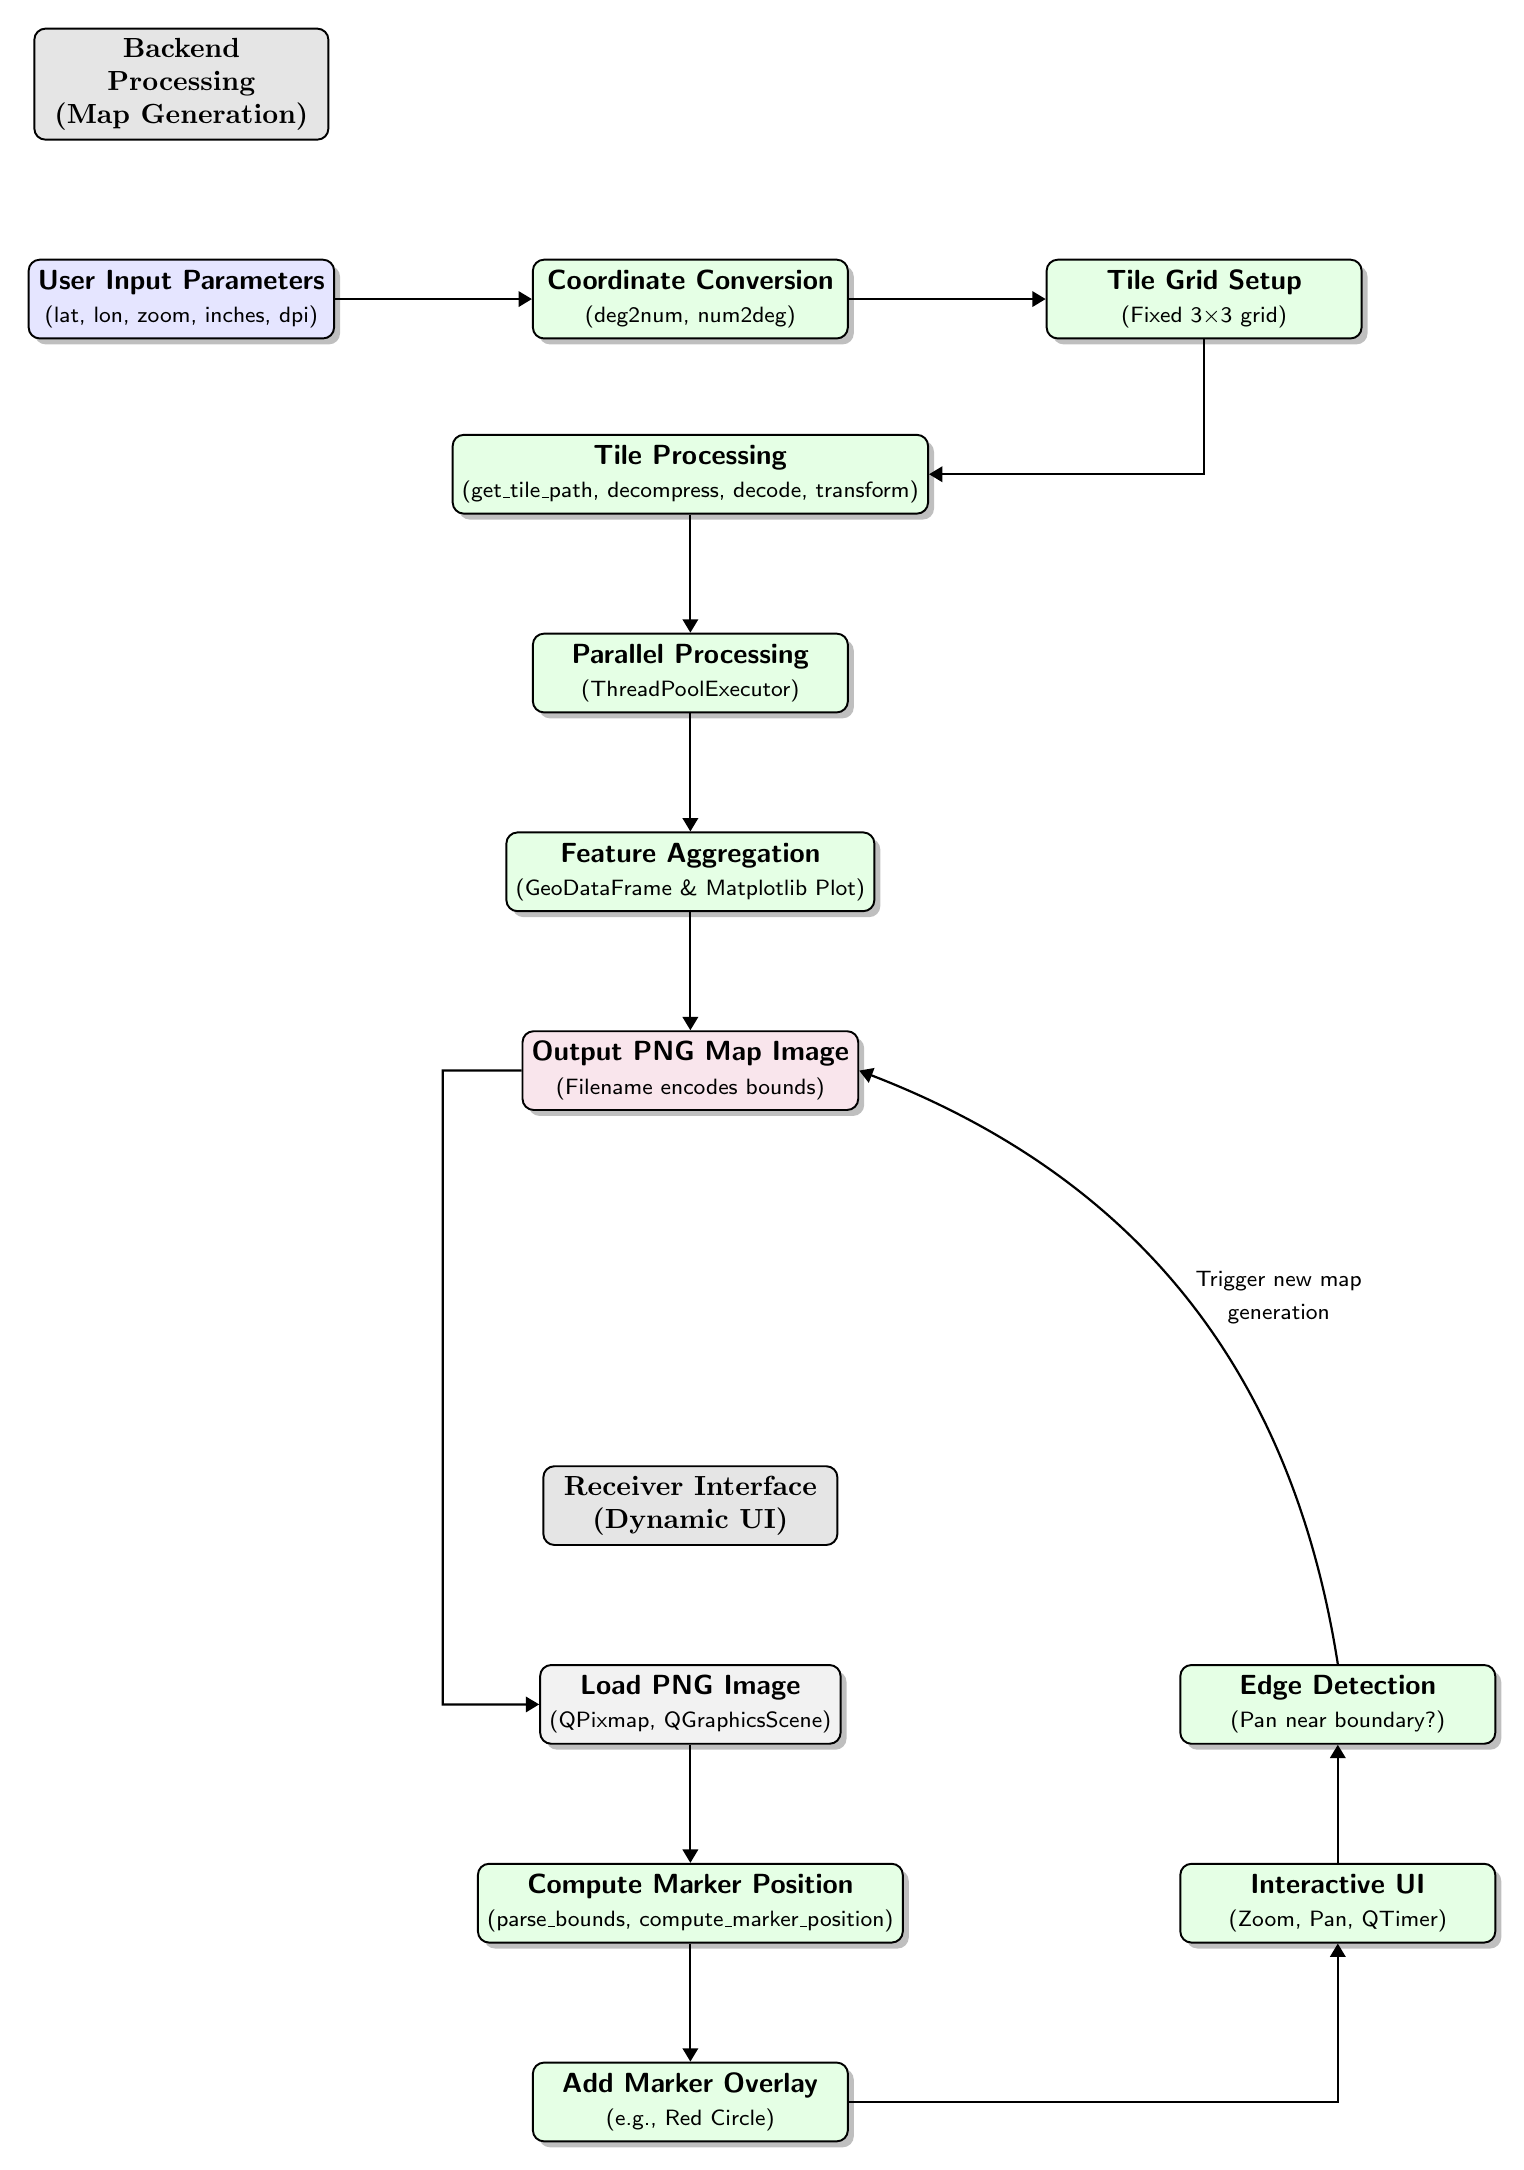
\begin{tikzpicture}[
  font=\sffamily,
  node distance = 1.5cm and 2.5cm,
  >=Triangle,  % Arrow tip
  line width=0.7pt,
  % Define block styles
  titleblock/.style={
    draw, 
    rounded corners,
    fill=gray!20, 
    text width=3.5cm, 
    minimum height=1cm, 
    align=center,
    font=\bfseries
  },
  inputblock/.style={
    draw,
    rounded corners,
    fill=blue!10,
    minimum width=3.6cm,
    minimum height=1cm,
    align=center,
    drop shadow
  },
  processblock/.style={
    draw,
    rounded corners,
    fill=green!10,
    minimum width=4cm,
    minimum height=1cm,
    align=center,
    drop shadow
  },
  outputblock/.style={
    draw,
    rounded corners,
    fill=purple!10,
    minimum width=4.2cm,
    minimum height=1cm,
    align=center,
    drop shadow
  },
  interfaceblock/.style={
    draw,
    rounded corners,
    fill=gray!10,
    minimum width=3.8cm,
    minimum height=1cm,
    align=center,
    drop shadow
  },
  % Arrows style
  connector/.style={
    ->,
    thick
  }
]

% -----------------------------------------------
% BACKEND SECTION TITLE
% -----------------------------------------------
\node[titleblock] (backendTitle) {Backend Processing\\(Map Generation)};

% -----------------------------------------------
% BACKEND FLOW
% -----------------------------------------------
\node[inputblock, below=of backendTitle] (inputParams) {
  \textbf{User Input Parameters}\\
  \footnotesize{(lat, lon, zoom, inches, dpi)}
};

\node[processblock, right=of inputParams] (coordConvert) {
  \textbf{Coordinate Conversion}\\
  \footnotesize{(deg2num, num2deg)}
};

\node[processblock, right=of coordConvert] (tileGrid) {
  \textbf{Tile Grid Setup}\\
  \footnotesize{(Fixed 3$\times$3 grid)}
};

\node[processblock, below=1.2cm of coordConvert] (tileProc) {
  \textbf{Tile Processing}\\
  \footnotesize{(get\_tile\_path, decompress, decode, transform)}
};

\node[processblock, below=of tileProc] (parallelProc) {
  \textbf{Parallel Processing}\\
  \footnotesize{(ThreadPoolExecutor)}
};

\node[processblock, below=of parallelProc] (featureAgg) {
  \textbf{Feature Aggregation}\\
  \footnotesize{(GeoDataFrame \& Matplotlib Plot)}
};

\node[outputblock, below=of featureAgg] (pngImage) {
  \textbf{Output PNG Map Image}\\
  \footnotesize{(Filename encodes bounds)}
};

% -----------------------------------------------
% RECEIVER SECTION TITLE
% -----------------------------------------------
\node[titleblock, below=4.5cm of pngImage] (receiverTitle) {Receiver Interface\\(Dynamic  UI)};

% -----------------------------------------------
% RECEIVER FLOW
% -----------------------------------------------
\node[interfaceblock, below=of receiverTitle] (loadImg) {
  \textbf{Load PNG Image}\\
  \footnotesize{(QPixmap, QGraphicsScene)}
};

\node[processblock, below=of loadImg] (markerPos) {
  \textbf{Compute Marker Position}\\
  \footnotesize{(parse\_bounds, compute\_marker\_position)}
};

\node[processblock, below=of markerPos] (addMarker) {
  \textbf{Add Marker Overlay}\\
  \footnotesize{(e.g., Red Circle)}
};

\node[processblock, right=3.5cm of markerPos] (interactiveUI) {
  \textbf{Interactive UI}\\
  \footnotesize{(Zoom, Pan, QTimer)}
};

\node[processblock, above=of interactiveUI] (edgeDetect) {
  \textbf{Edge Detection}\\
  \footnotesize{(Pan near boundary?)}
};

% -----------------------------------------------
% ARROWS AND CONNECTIONS
% -----------------------------------------------

% Backend flow
\draw[connector] (inputParams) -- (coordConvert);
\draw[connector] (coordConvert) -- (tileGrid);

% A small vertical drop from tileGrid to tileProc
\draw[connector] (tileGrid.south) |- (tileProc.east);

\draw[connector] (tileProc) -- (parallelProc);
\draw[connector] (parallelProc) -- (featureAgg);
\draw[connector] (featureAgg) -- (pngImage);

% Connection from PNG to receiver flow
\draw[connector] 
  (pngImage.west) -- ++(-1,0) % step 1: go left
                     -- ++(0,-8.05) % step 2: go down
                     -- ++(1,0)  % step 3: go right
                     -- (loadImg.west); % step 4: connect to target

% Receiver flow
\draw[connector] (loadImg) -- (markerPos);
\draw[connector] (markerPos) -- (addMarker);

\draw[connector] (addMarker.east) -| (interactiveUI.south);
\draw[connector] (interactiveUI) -- (edgeDetect);

% Feedback arrow from Edge Detection back to PNG creation
\draw[connector, bend right=30] (edgeDetect.north) to node[midway, right, align=center]
{\footnotesize Trigger new map\\ \footnotesize generation} (pngImage.east);

\end{tikzpicture}
\end{document}
